\section{Navigation}\label{sec:navigation}
There are several different navigation structures that are recommended by Google, the most significant ones being, the navigation drawer and fixed tabs. Both of the design patterns are suitable for switching views frequently, and have multiple top level views. 
On Google's developer page for Android it says \textit{``Use the navigation drawer if you have more than 3 unique top-level views.''}\cite{guidelines-navigationdrawer}, this supports our decision of implementing the navigation drawer in our application. The navigation drawer will also make the application easier to expand with more functionality, and we do not sacrifice vertical space as we would have done with a dedicated tab bar. Vertical space is very important for our application because it is used to display the details of a recipe, search results, and many other things.

\subsection{Navigation drawer}
The navigation drawer is a design that allows the user to navigate to any top level view from any context, which means that even if the user is on a lower level view, the user can just expand the navigation drawer to reach the top level views. 
The navigation drawer has an option to change which side it should be expanded from, but it is typically expanded from the left side of the application.
\begin{figure}[H]
\centering
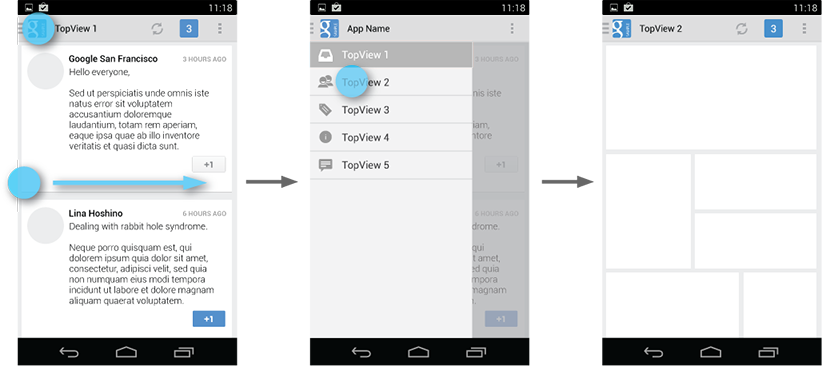
\includegraphics[width=0.9\linewidth]{img/screenshots/navigation_drawer_overview.png}
\caption{Navigation drawer overview\cite{guidelines-navigationdrawer}.}
\label{fig:navigationdrawer}
\end{figure}
There are two different ways of expanding the navigation drawer, the consistent one being swiping from the left edge of the screen to the centre, this can always be achieved no matter the context. 
The second one being pressing the button in the top left corner, this option is not consistent since the button changes both appearance and functionality depending on which view level the user is on. 
If the user is on a top level view, the button's appearance will consist of three thick lines, and \autoref{fig:navigationdrawer} shows that if pressed the navigation drawer will expand.
If the user is entering a lower level view, it will change the button's appearance to an arrow pointing left, and its functionality to be a return button, that if pressed will navigate the user back to the top most view. 
Each item in the navigation drawer navigates to different top-level pages in the application or typical main actions like sign-in/sign out.

\subsection{Application navigation}
In our application we expect to implement six top level views ingredient search, recipe search, favourites, shopping list, settings, and sign-in/sign out. 
Our application only has one lower level view which is the display of a recipe, it is a lower level view because it is only accessible through other views.
Some views or actions in the application might require the user to be signed in, for them to be available. 
Like the favourites view, which displays the recipes that the user has favourited.
If the user is not signed in when entering the favourite view, they are prompted with a text asking them to sign-in, this should always happen in the case the user tries to use user-functionalities. 
In the bottom of the navigation drawer we plan to add an item with the action of signing in, or signing out the user, it is located in the bottom of the navigation drawer to signalise its difference with the other items in the navigation drawer.
\begin{figure}[H]
\centering
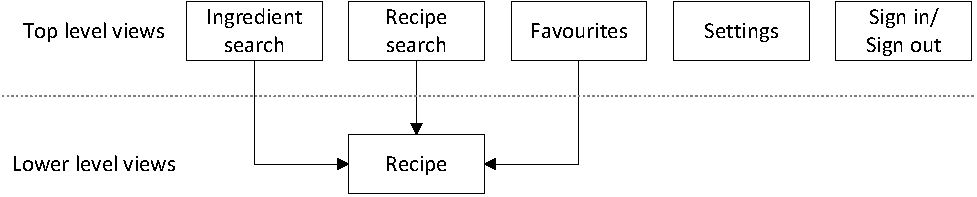
\includegraphics[width=1.0\linewidth]{img/navigation.pdf}
\caption{Navigation view flow.}
\label{fig:navigationViews}
\end{figure}
\autoref{fig:navigationViews} shows the views that are accessible in the application, and the navigation flow between the views. 
It can be seen that to reach the recipe view you have to go through either ingredient search, recipe search or favourites. It should be noted that it is always possible reach to top level views, no matter the context the user is in.
